\documentclass[12pt, conference, final, a4paper, onecolumn, compsoc]{IEEEtran}
% Font size onecolumn or twocolumn Use draft for notes or final for no spacing

% Includegraphics
\usepackage{graphicx}
% Bibliography
\usepackage{natbib}
% Figure positions
\usepackage{float}
% Wrapping figures
\usepackage{wrapfig}
% Wrapping URLs
\usepackage[hyphens]{url}

\begin{document}


\title{Using AI to Detect Malware in Object Storage} \author{Author: Matthew
  Battagel, Supervisor: Theodoros Spyridopoulos} \markboth{Cardiff University -
  CM3203 - Final Report}{}
\maketitle{}

\subsection*{Acknowledgments - }
% Remove section from TOC
\addtocontents{toc}{\protect\setcounter{tocdepth}{-1}}

I would like to extend my sincere gratitude to my supervisor Theo, my colleague
Harry, friends, family, and Lois for their unwavering support and encouragement
during my project. Their combined expertise and guidance provided were critical
in the shaping and execution of the project. I am truly grateful to all of them
for their contributions.

\bigskip

\begin{abstract}
  Lorem Ipsum
\end{abstract}

\pagebreak

% Problem and background Understanding of the problem and the aims and
% objectives of the project Awareness of the background of the problem

% Detailed analysis of the problem, suitability of approach towards solving the
% problem Solution to the problem Approach and design Solution, implementation
% Use of and justification for appropriate tools/methods

% Evaluation Testing and validation Critical appraisal of results

% Achievement of agreed overall deliverables given in the initial plan for the
% final report (or a justified modification of these) Communication and project
% management skills Written communication skills Project planning, control and
% reflection Interaction and work with the supervisor


% Contents
\tableofcontents{}


\section{Introduction}
\subsection*{Overview}
% Data growth and object storage
The exponential growth of data generation has made data storage an increasingly
important aspect for both individuals and organizations alike. Object storage
has emerged as a promising solution due to its ability to store vast amounts of
unstructured data in a cost-effective and scalable manner. Unlike traditional
storage techniques, object storage stores data as objects with related metadata
and unique identifiers, allowing for efficient and cheap storage within buckets.

% TODO Re-word last part

% Market and competition
One of the most widely used object storage platforms is Amazon S3, which
provides a highly scalable and reliable solution for storing data. However, an
open-source alternative called MinIO has emerged as a promising contender,
providing similar features to Amazon S3 while giving customers greater control
over their data. MinIO is written in Go and is available for free under the
Apache License 3.0 or, for commercial and enterprise purposes, at a reduced cost
compared to Amazon S3. \citep{minio-pricing}. MinIO offers a wide range of
features, including high performance, data replication, encryption and erasure
coding \citep{minio}. Most importantly, MinIO is designed to scale out
horizontally to ensure that it can handle the demands of large-scale
applications.

% Scalability
Scalability is made simple by allowing multiple types of hardware platforms to
work together in separate nodes each with their own compute and storage. This is
extremely attractive for customers who want to utilises their existing hardware
without being tied down to a specific provider. This also applies for customers
looking to migrate their data from Amazon S3 to cheaper solution without
compromising on the high performance, reliability and scalability of the S3
platform.

% Downsides
While MinIO is a great alternative to Amazon S3, it does not offer any form of
malware detection integration. This could put customers off from choosing MinIO
as a viable platform to migrate to from Amazon S3 or leave existing users data
vulnerable to malware attacks. This project aims to address this issue by
integrating a malware detection system into MinIO. An important goal for the is
to negatively impact the scalability or performance as little as possible so
that MinIO is still an effective alternative to Amazon S3.

\subsection*{Motivation} % Why am I trying to add malware detection for object storage?
% TODO Can I say about HPE? Or shall I say its for the good of the world

Due to the high amount of unstructured data expected to be both written and read
to the object store, there are increased risk of encountering malicious files.
Therefore malware detection within object storage is crucial in modern cloud
storage scenarios. Most popular off-the-shelf object storage platforms, such as
AWS, already have integrated third-party antivirus software, such as ClamAV and
Sophos \citep{amazon-md}, to mitigate security risks. MinIO on the other hand is
vulnerable to malware attacks as it currently does not have any native antivirus
integration. This forces customers who require complete virus protection to
either not use MinIO or to use potentially costly third-party software. As
antivirus scanning is inherently resource intensive, if the software is
integrated incorrectly, it could reduce the ability for the storage solution to
scale horizontally which negates one of the major benefits of object storage.
The purpose of this project is to implement malware detection within MinIO while
being mindful to not impact the scalability or performance of the platform.

\subsection*{Project Aims} % What the project aims to achieve

This project aims to supply an end-to-end solution for detecting malware within
the MinIO object storage platform with three main requirements. The solution
should be able to detect the latest uploads to the object store and scan them.
It should be able to perform this function without significantly impacting the
performance of the object store. The solution should also scale alongside MinIO
to ensure that it does not bottleneck the object store at high loads. These main
three aims can be quantified so that an accurate evaluation of the solution can
be made at the end of the project.

\begin{itemize}
  \item Detection of malware within the object store should match 100\% of the
        malware detection rate as the stand-alone antivirus.
  \item Performance of the solution to be within 10\% of the performance of the
        stand-alone object store, MinIO.
  \item Retain the previous metric while both increasing the available resources
        and changing the platform.
\end{itemize}

% TODO Maybe not here?
\subsection*{Milestones} % Breakdown of key targets through project

There are many key milestones that can be used to measure the progress of the
project through the duration of its implementation. It is worth noting that
these milestones were created before the implementation of the solution and
therefore are subject to change.

% TODO I am talking about a lot of specific things here. Do they know what it
% means?
\begin{itemize}
  \item Setup local ClamAV instance
  \item Setup local MinIO instance
  \item Setup local Kafka instance
  \item Detect PUT message on Kafka
  \item Read JSON of message to find bucket and object path
  \item Create AV manager service in GoLang
  \item Request GET on Object using message data
  \item Scan Object using Clamd
  \item Act on result of scan - Add tags, "scanned", "date\_scanned"
  \item Configuration file using viper
  \item Add metric collection with Prometheus
  \item Add structured logging with zap
  \item Create Database of Audit Logs with postgresql
  \item Termination of connections to services
  \item Create tests for each package using mockery

  \item Prepare for Kubernetes deployment with k3d
  \item Containerise Aegis with Docker
  \item Automatically configure and start MinIO, Kafka, Clamd, Postgresql,
        Prometheus and Aegis with Helm
  \item Port forward MinIO out of the cluster
  \item Load balancing / performance analysis for Clamd
  \item Expose Postgresql and Prometheus for analytics
  \item Prepare configurations for demo, release etc
  \item Clean-up version control and write readme.me
\end{itemize}

These milestones can be broken down even further into smaller tasks. These are
best represented in Gantt / burndown charts which can be found in the appendix.
% TODO Reference

\section{Background}

% background should be more previous research material etc. Include competition
% and potential software to use e.g. ClamAV, MinIO. Include the first things you
% find when googling the same topic as diss.

% Where to put background info on object storage and malware? Not sure
    %

% Insert background material
    %

\subsection*{Amazon S3 Malware Detection} % How does amazon do it?

As MinIO's largest competitor, this project draws a lot of inspiration from
Amazon S3s integrated malware detection blog page \citep{amazon-md}. The blog
explains Amazons current approach for managing malware detection within their
service. Amazon S3 uses a combination of ClamAV and Sophos as their third-party
scanning engines due to their out-of-the-box nature. Amazon then gives you the
option to use either of these engines or both. The blog goes on to describe the
three main interaction mechanisms that Amazon S3 uses to flag files for
scanning. Firstly, an API endpoint would be provided to handle all uploads. This
forms a queue of uploads which are then scanned before entering the bucket.
Next, event-driven scanning is used keep track of all regular file uploads. The
antivirus will then scan each file after they have been written to the bucket.
Finally, retro-driven scanning is used to scan all existing files within the
bucket. The user then has the flexibility to define what types of files should
be scanned including defining time windows. This blog has given some useful
methodologies of how to keeping track of both incoming and previously scanned
files. Creating a system that can match these methods is important for offering
a matching level of scalability and security within MinIO.

% Talk about standard flow and two bucket flow - useful in designing

% Amazon use stub files

\subsection*{} % How does signature detection work?


\subsection*{} % Best ways of implementing AV into a micro-service?


\subsection*{} % How does ClamAV work? What is clamd

% Malware Artificial Intelligence Object Storage Context

\section{Specification and Design}

\subsection*{Specification}

The specification for this project is to help guide the project to fufill the
aims set out in the previous section. The specification is broken down into
three main sections; functional requirements, non-functional requirements and
constraints.

\subsubsection*{Functional Requirements}

Functional requirements are


% TODO Say about we need to keep up so that people are not waiting and the
% system does not get behind. Maybe use metrics to show how we DO keep up?
    %

% TODO What to do with infected files TODO What to do with files that are not
% scanned TODO How to remove infinite loops TODO How to handle large files TODO
% How many AVs could be used? TODO Security issue of not checking put tagging

\subsubsection*{Non-Functional Requirements}

Non-functional requirements are

\subsubsection*{Constraints}
\paragraph{}

The constraints are the limitations that the solution must adhere to. The main
constraint of the project is the strict time limit given to the project. There
are a total of 12 weeks to achieve a production ready product which will greatly
limit the scope of the project. This means accurately prioritising the features
that are most important to the project while also balancing the time spent to
implement them. The second constraint is the limited resources available to the
project.


Another constraint of the project is that all the external software used must be
open source / available for commercial use under license or fee. This is to
ensure that the project is legally viable if the solution was to be used
commercially.


The final constraint is that the solution must

% TODO final constraint


\subsection*{Architecture}

    \paragraph{}
    Given the specification above, various potential architectures can be
    created and evaluated. An optimal design will then be chosen based on which
    design fits the specification best.

    % TODO Crop the diagrams to remove the white space

    % Post-Write
    \subsubsection*{Design 1 - Post-Write}
    \paragraph{}

    This design makes use of the performance benefits of MinIO by allowing puts
    to be initially written to the bucket without being scanned. The design then
    uses a event queue compatible with MinIO to keep track of all the files that
    have been uploaded. The queue is then used to trigger a scan of the file
    once an antivirus is available. The design is shown in figure
    \ref{fig:postWriteArch}.

    \begin{wrapfigure}{r}{0.45\textwidth}
      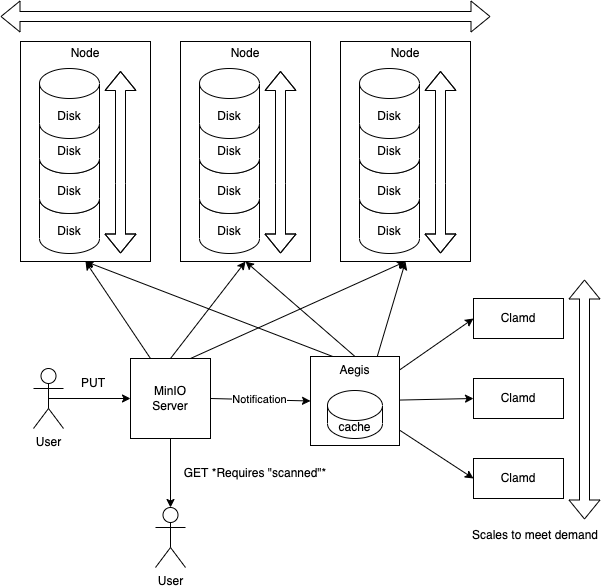
\includegraphics[scale=.4]{diagrams/post-write.png}
      \caption{Post-Write Architecture}
      \label{fig:postWriteArch}
    \end{wrapfigure}

    This design has many benefits over other potential implementations. Firstly,
    it uses the storage provided by MinIO to store all incoming files without
    having to manage a separate storage solution. This removes a lot of
    complexity from the solution by not having to account for a number of
    failure conditions that could occur with a high availability, production
    ready storage solution. For example, the solution would not be responsible
    for handling partial writes, loss of data, or data corruption. Removing this
    responsibility allows the solution to focus on the core functionality of the
    project, the scanning of files, which is essential for keeping the project
    within the time constraints.

    Secondly, the design also makes use of the integrated event queue provided
    by MinIO. This again removes responsibility from the solution by differing
    the scalability and reliability requirements of an event queue to MinIO.

    % TODO DO THEY KNOW WHAT AEGIS IS? TODO Change the diagrams to be service
    % ambiguous

    Lastly, having Aegis dispatch the files to a scalable number of antivirus
    scanners allows the solution to scale to meet the demands of the system.
    This meets a key requirement as the solution is expected to have the
    capacity for a large number of operations. This method does require the use
    of a load balancer to effectively distribute the load across the available
    antivirus scanners.

    The design also has a number of drawbacks. Firstly, the design still
    requires a small about of cache to temporarily store the object when it is
    being dispatched to the antivirus. Provisioning of this cache has to be
    large enough to handle the largest file possible to be uploaded to the
    object store. In reality, this cache would be provisioned even larger to
    allow for the temporary storage of multiple objects while multiple scans are
    being performed asynchronously. In addition, the cache needs to be large
    enough to ensure that the system does not become overwhelmed by the number
    of objects being scanned as the system scales. This is a minor issue as
    store capacity is cheap and the provisioning of the cache easy to scale up.
    Additionally, a higher priority can be given to scaling up and out antivirus
    scanners to ensure that the smallest number of files are being cached, while
    bring scanned, at any point.

    % TODO Do they know what get/put is? TODO Do they know distributed storage
    % topologies?

    The second drawback is that, for each event, Aegis makes a get request for
    the object to be scanned. This effectively doubles the number of requests
    made to the object store. This also means that Aegis must have the ability
    to get any file expected to be scanned and therefore must have access to the
    whole storage network. The impact of this drawback is mitigated as the
    solution is expected to be deployed on the same network as the object store
    which should reduce the latency of each request made by Aegis. However, this
    still leaves MinIO to handle twice as many requests with the performance
    loss being noticed mainly on more distributed storage topologies.

    Thirdly, the design only allows for a single Aegis instance to dispatch all
    incoming objects to available scanners. This is a potential bottleneck for
    the system as this instance could become overwhelmed by the number of
    requests it is receiving. This is a minor issue as the dispatching of
    objects to scanners is not as performance intensive as other areas of the
    solution, such as the actual scanning, and therefore it is not expected to
    be a major bottleneck.

    Lastly, any object uploaded to the store will have a certain period of time
    where it remains unchecked. In this time, the user could potentially
    download an unscanned object or the object could cause harm to the store
    before it is detected. Although the handling of infected objects is out of
    scope, in an actual implementation of the solution, the user could be made
    unable to download unscanned objects until they have been scanned.

    % TODO AWS does this with S3 events 'standard flow'

    \subsubsection*{Design 2 - Upload Queue}
    \paragraph{}

    % TODO More explanation here?
    This design created a wrapper around MinIO that the user interacts with
    instead of MinIO. This means that all puts go through Aegis before being
    uploaded to the object store. The design is shown in figure
    \ref{fig:uploadQueueArch}.

    \begin{wrapfigure}{r}{0.45\textwidth}
      \centering 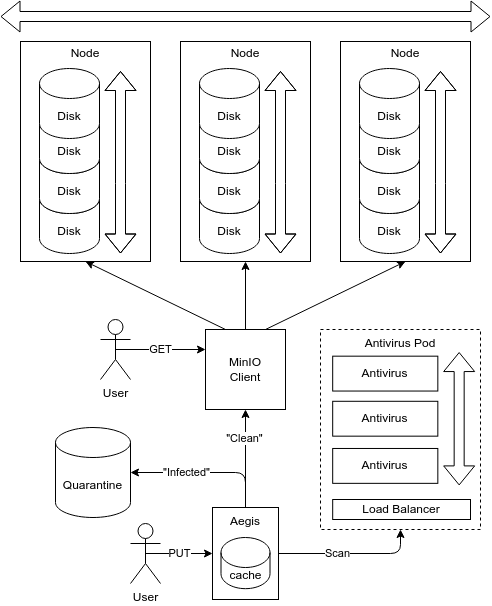
\includegraphics[scale=.4]{diagrams/upload-queue.png}
      \caption{Upload Queue Architecture}
      \label{fig:uploadQueueArch}
    \end{wrapfigure}

    The main benefit of this design is that the user interacts only with Aegis
    when uploading files. This means that all incoming files can be stored
    within a temporary storage before ever entering the object store. This
    offers the best protection against malicious files as the user cannot ever
    download an unscanned or infected file as it is never uploaded to the object
    store. Infected files can then either be deleted or moved to a separate
    quarantine store for analysis.

    This designs main advantage also comes with a major drawback. This design
    requires Aegis to handle the full throughput of all the puts to the system.
    Aegis then has the full responsibility of being available to all puts and,
    in a failure scenario, to handle the recovery of the system. Additionally,
    the cache provisioned must be large enough to handle the largest files at
    maximum throughput with extra room for unexpected delays. This negatively
    affects the scope of the project by requiring the solution to prioritise
    features that are already covered by MinIO.

    % TODO Cover mitigation

    % TODO is this already covered?
    Because MinIO is dependent on Aegis to handle the puts, MinIO must wait to
    be passed incoming objects sequentially after Aegis has finished processing
    the previous object. This removes the potential for aggregate performance
    where

    % TODO Talk about how AWS uses this method 'Two Bucket System Flow'

    \subsubsection*{Design 3 - Write Interception}
    \paragraph{}

    % TODO Edit diagram to show quarantine?

    Design three is very similar to the second design, however, instead of
    wrapping outside the MinIO service, it intercepts the writes from the client
    before objects are written to the object store. With this interception,
    Aegis can scan the object and decide whether to allow the object to be
    written to the store or to quarantine the object. The design is shown in
    figure \ref{fig:writeInterceptArch}.

    \begin{wrapfigure}{r}{0.4\textwidth}
      \centering 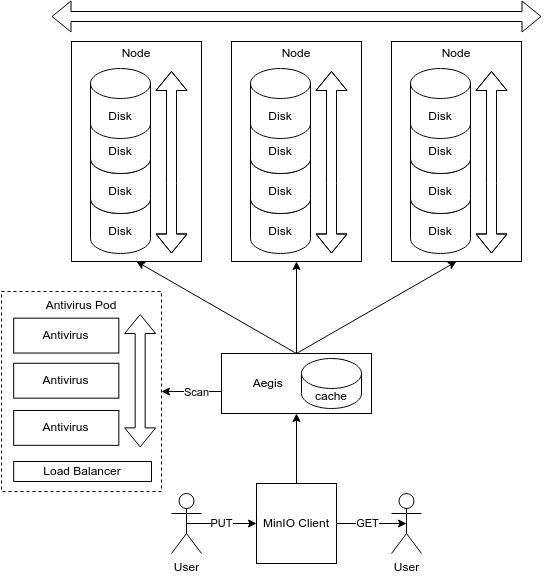
\includegraphics[scale=.3]{diagrams/write-intercept.png}
      \caption{Write Interception Architecture}
      \label{fig:writeInterceptArch}
    \end{wrapfigure}

    This design has similar benefits as the second design. It offers the most
    protection against malicious files by never allowing either unscanned or
    infected objects to be stored in the object store. However, it also has
    similar drawbacks. This is because Aegis is still in sequence with MinIO
    meaning that for optimal throughput, Aegis would need to match the
    performance of MinIO.

    Similar to the upload queue design, this design also requires Aegis to have
    a large cache to handle the largest files at maximum throughput. This cache
    must also be large enough to handle the number of objects being put by MinIO
    into the store. This issue cannot be mitigated without the risk of
    compromising performance at increased loads.

    However, this design does have an advantage over the second design as there
    is less responsibility placed on Aegis to be as failure tolerant. MinIO is
    still directly responsible for accepting objects into the store and
    therefore is still responsible for the recovery of the system in a failure
    scenario. This allows the scope to focus on more related features to malware
    scanning.

    % TODO Encrypted???

    \subsubsection*{Design 4 - Per Node}
    \paragraph{}

    % TODO More?
    The final design distributes Aegis onto each node in the object store. This
    means that each node has a local instance of Aegis that is responsible for
    scanning objects before they are written to the store. The design is shown
    in figure \ref{fig:perNodeArch}.

    \begin{wrapfigure}{r}{0.5\textwidth}
      \centering 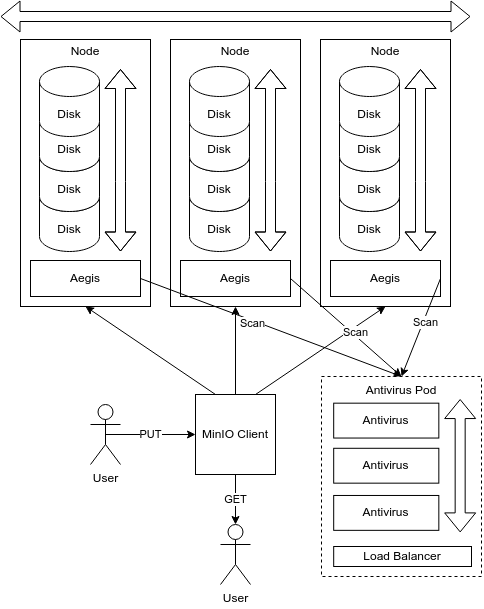
\includegraphics[scale=.3]{diagrams/per-node.png}
      \caption{Antivirus per Node Architecture}
      \label{fig:perNodeArch}
    \end{wrapfigure}

    This design makes use of the distributed nature of MinIO to match the demand
    when scaling out the system. As more nodes are added, more Aegis instances
    are added to handle the increased scanning demand. This removes the need for
    having a cache repository as Aegis already has access to the files that need
    scanning. By removing this single point of failure, in theory, the system
    only relies on the antivirus pod to be able to scale out on its own.

    Independent scaling of the antivirus pod allow for efficient usage of
    available hardware. A simple load based auto-scaler can be used to scale the
    number of pods based on the current load. This allows for the system to
    flexible scale with the demand of the system and to reduce usage of valuable
    resources, such as power. There is also the opportunity to use intelligent
    scaling techniques to predict the load on the system and prematurely scale
    the system to meet the demand. For example, to scale the number of pods
    depending on the time of day or the day of the week.

    % TODO Explain MinIO terms
    The major drawback of this design is that it replies on the ability to scan
    whole files by only using data on a single node. In actual implementations,
    MinIO makes use of erasure coding to add increased redundancy to the store
    \citep{minio-erasure}. Erasure coding splits objects into multiple parts
    known as blocks, and then calculates corresponding parity blocks. These data
    and parity blocks are then distributed among all nodes in the system
    allowing for on-the-fly data recovery even with the loss of multiple drives
    or nodes . This means that the Aegis instance on each node only has access
    to the part available on their node and therefore will not be able to
    reconstruct the whole file for scanning. This makes this design unsuitable
    for MinIO as it erasure coding is one of its key features.


    \subsubsection*{Optimal Design}

    % TODO what if admin wants to store malware? Who are we to judge?
    % Flexibility Security Performance Scalability Resource use
    %

    Given the above evaluations of each design, design one best suits the
    requirements and constraints of the project. It makes the most use of the
    existing features that MinIO provides to handle failure scenarios and to
    scale out. This also means that this design has less critical responsibility
    and will better fit the scope constraints allowing for more time to be spent
    on supplementary features, such as testing, logging, and metric collection.
    Because of this, the produced solution will be closer to production-ready
    than the other designs.

    This design keeps the user in control by giving them the ability to store
    unscanned files / known malware without wasting resources on a scan.
    Protection can be added per bucket therefore a user could have a known
    malware bucket and a clean bucket within the same object store. This allows
    for the system to be more flexible and to be able to handle more use cases.
    Designs two and three would not be able to handle this use case as they both
    scan all objects before they are written to the store.

    The size of the cache required is smaller than all other designs as it only
    needs to store the objects actively being scanned. This is in opposition to
    upload queue and write interception designs as they have to be prepared to
    handle the full demand placed on the store. This makes design one the most
    lightweight of all the designs which should lead to a smaller resource
    footprint

    \section{Implementation}
    \subsection*{Event Queue}
    % Kafka

    \subsection*{Packaging}

    \section{Results and Evaluation}
    % Evaluate against specification Compare to MinIO Find figures like average
    % scan Compare local vs cluster
    \subsection*{}

    \section{Product Issues / Future work} % What you would do next time
    \subsection*{}

    \section{Conclusions}
    \subsection*{}

    \section{Reflection on Learning} % Fuck knows
    \subsection*{}

    \section{Appendix}
    % TODO Add figues and tables to appendix
    \bibliographystyle{cardiff} \bibliography{references}

  \end{document}

  % TEMPLATED
  % \begin{figure}[!ht]
  %   \centering \includegraphics[scale=.55]{assets/extracred}
  %   \caption{Bouncing and pitching motion as a function of time}
  %   \label{fig:bounceAndPitch}
  % \end{figure}

  % \begin{table}[!ht]
  %   \begin{center}
  %     \caption{Calculated values}
  %     \label{tab:calculated}
  %     \begin{tabular}{|c|c|}
  %       \hline
  %     \end{tabular}
  %   \end{center}
  % \end{table}

  % Appendix \onecolumn \textwidth=456pt \paperwidth=577pt \hoffset=-30pt
  % \newpage
  % \newpage
  % \clearpage


  % \pagestyle{headings}
  % \section{Appendix A}
  % \centering Heading \footnotesize

  % \normalsize

  % \csvautolongtable{assets/vibProj.csv}
  %

  % I DONT THINK THIS IS WHAT THEY MEANT BY BACKGROUND
  % \subsection*{Malware}
    %
  % Malware is a type of software designed to harm or exploit computer systems,
  % networks, and users. It includes a wide range of harmful programs, such as
  % viruses, worms, Trojans, ransom-ware, spyware, and adware. Malware can be
  % used to steal sensitive information, gain unauthorized access to systems,
  % damage or destroy data, and perform other malicious activities. Malware can
  % be distributed through various channels, such as email attachments,
  % malicious web-sites, software downloads, and infected removable media. It is
  % a serious threat to computer security and can cause significant damage to
  % storage devices if left untreated.
  % % TODO And has the potential to be laying dormant inside peoples computers
%
    %
  % Malicious files can be particularly risky for storage devices in cloud
  % environments due to their shared nature. In a cloud storage environment,
  % multiple users and applications can access and store data on the same
  % physical storage infrastructure. This means that an infected file can
  % quickly spread and infect other files and users, compromising the security
  % and integrity of the entire system. Moreover, cloud storage providers may
  % not be able to isolate and contain malware as easily as with traditional
  % storage systems. As a result, cloud storage users need to be extra vigilant
  % and take proactive measures, such as implementing antivirus software,
  % regular backups, and secure access controls, to mitigate the risks of
  % malware infections.
%
  % \subsection*{Anti-Virus}
  % % Create a connection between paragraphs here. Include Citation
    %
  % In the context of modern IT solutions, ensuring robust security measures is
  % crucial to guarantee reliable operations and safeguard data against threats.
  % Companies can face severe penalties, up to ???, for failing to comply with
  % data protection regulations in the event of a breach. Therefore, it is
  % imperative that IT products offer comprehensive security features, mainly
  % including built-in antivirus capabilities, to protect against malicious
  % attacks and prevent data loss.
%
    %
  % Modern Anti-Viruses mostly work using a combination of signature-based and
  % heuristic detection methods. Signature-based detection works by comparing
  % the file being scanned against a database of known malicious file
  % signatures. If a match is found, the file is flagged as malicious. This
  % method is effective at detecting known malware, but it is not effective at
  % detecting new or unknown malware. Heuristic detection, on the other hand,
  % works by analyzing the behavior of the file being scanned and comparing it
  % against a database of known malicious behaviors. This method is more
  % effective as it looks at practices used by malware, such as common imports,
  % and therefore has potential to detect previously unknown malware.
%
  % % EXPLAIN HOW MACHINE LEARNING CAN BE USED?? Tie it into next paragraphs
%
  % \subsection*{Artificial Intelligence}
  % % What is AI? Why use AI? Is it better than regular detection? How does this
  % % affect our definition of malware and antivirus?
%
    %
  % % SUBSEQUENTLY EXPLAIN WHAT AI IS?
%
  % \subsection*{Object Storage}
    %
  % Object storage is a type of data storage architecture that manages data as
  % discrete units known as objects. Each object contains data, metadata
  % (information about the object), and a unique identifier that enables it to
  % be located and retrieved. Object storage systems are designed to handle
  % large amounts of unstructured data, such as files, images, videos, and other
  % multimedia content and have become increasingly popular in recent years with
  % a compound annual growth rate of 13.6\% \citep{object-storage-market}.
%
    %
  % Unlike traditional storage architectures like file or block storage, object
  % storage does not organize data in a hierarchical directory structure or use
  % fixed-sized blocks. Instead, it allows data to be stored and accessed
  % independently of the underlying physical storage infrastructure. This makes
  % it easier to scale storage capacity and performance, as well as to implement
  % features like data replication, versioning, and encryption. Object storage
  % is often used in cloud computing environments, where it is a popular option
  % for storing and managing data in distributed systems.
%
%
  % \subsection*{MinIO}
    %
  % MinIO is a high-performance, open-source, distributed object storage system
  % that is designed to be an alternative to Amazon S3. It is S3 compatiable
  % allowing for almost instantanous migration from Amazon to MinIO. MinIO is
  % also designed to scale horizontally and can be deployed on a wide variety of
  % hardware and software platforms \citep{minio}. It is written in Go and is
  % available under the Apache License 2.0 \citep{minio-repo}. MinIO has several
  % features that make it an attractive choice for cloud-native applications. It
  % is fault-tolerant, with data being automatically distributed across multiple
  % drives and servers (erasure) to ensure high availability. Additionally,
  % MinIO is highly performant, with a focus on optimizing for SSDs and NVMe
  % drives \citep{minio}.
%
    %
  % Currently, MinIO does not provide built-in antivirus capabilities. This
  % means that users must rely on third-party antivirus software to protect
  % their data from malware. However, this can be a challenge for users who want
  % to use MinIO in cloud environments, as antivirus software is often
  % incompatible with cloud-native applications. This is because antivirus
  % software is designed to run on a single machine and is not designed to scale
  % horizontally. As a result, antivirus software is not well-suited for
  % cloud-native applications, which are often deployed in distributed
  % environments. Moreover, antivirus software is often resource-intensive and
  % can slow down the performance of cloud-native applications if scalability is
  % not properly considered. This is particularly problematic for cloud-native
  % applications that require high performance, such as video streaming and
  % machine learning.
%
    %
  % Adding an in-built antivirus capabilities to MinIO would allow users to
  % protect their data from malware without having to rely on third-party tools.
  % This would also allow users to run antivirus software in a cloud-native with
  % scalability and performance in mind. In this report we will discuss
  % different approaches that can be taken to embed an antivirus engine into
  % MinIO and evaluate their performance and scalability.
%
  % \subsection*{ClamAV}
  % % Describe inner workings!?!?! Open-source
%
    %
  % Open-source antivirus software is a popular choice for cloud-native and
  % distributed applications. This is because open-source software is often
  % free, which makes it a cost-effective option for users. Additionally,
  % open-source software is often more customizable and flexible than
  % proprietary software, which makes it easier to integrate into cloud-native
  % applications. Open-source software is also often more secure than
  % proprietary software, as it is often reviewed by a large community of
  % developers and users.
%
    %
  % % TODOCHECK does it focus on distribution??
  % One of the most popular open-source antivirus software is ClamAV. It is
  % written in C and is available under the GNU General Public License
  % \citep{clamav-repo}. ClamAV is designed to be lightweight and fast, with a
  % focus on distributed and scalable scanning. ClamAV uses a combination of
  % signature-based and heuristic detection methods as mentioned earlier with a
  % reported accuracy of ???. It uses an open-source database of known malicious
  % files and behaviors which is updated regularly by the ClamAV community.
%
    %
  % % TODOCHECK is this what we do in the end?? Can we use AI to make it better?
  % % How?
  % For prototype implementation and benchmarking of the system architecture, we
  % will use ClamAV as our antivirus engine. This can then be replaced or
  % upgraded with a more advanced antivirus engine that utilises AI.
